\section{Exercise 2: An application of MCFP: rectilinear planar embedding}

\begin{figure*}
  \label{fig:rect-emb}

  \begin{center}
  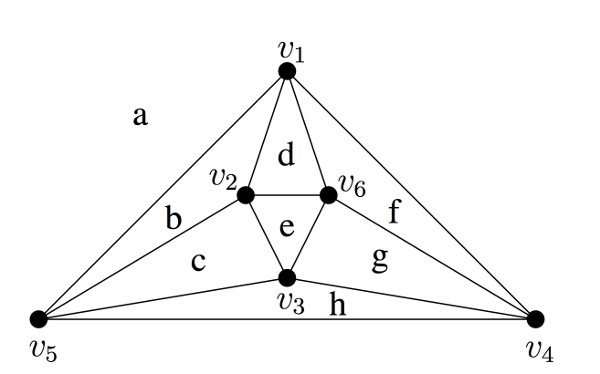
\includegraphics[scale=0.3]{img/fig2b.png}
  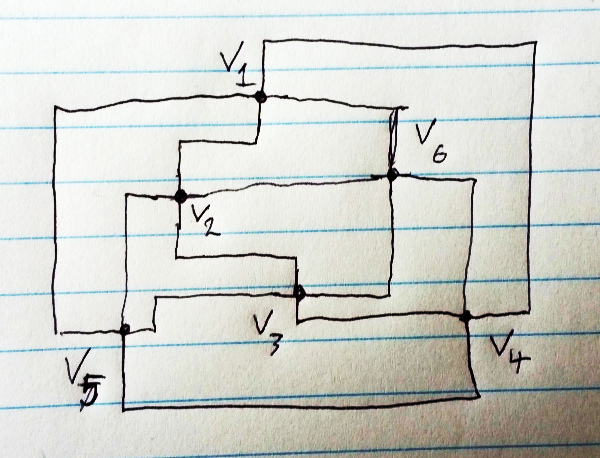
\includegraphics[scale=0.3]{img/ex21.png}
  \end{center}
  
  \caption{Figure 2 (b) from the practice set (left) and a sketch of its rectilinear embedding (right).}
\end{figure*}

\subsection{Exercise 2.1}

Listing only the values of $z_{fg}$ where $f$ and $g$ share an edge,
and on the values of $x_{vf}$ where $v$ is a corner edge of $f$.
\begingroup
\newcommand\zfg[3]{z_{ #1 #2} &= #3}
\newcommand\xvf[3]{x_{ #1 #2} &= #3}
\begin{align*}
  \zfg a b 0 \\
  \zfg a c 0 \\
  \zfg a e 0 \\
  \zfg b a 2 \\
  \zfg b c 1 \\
  \zfg b d 1 \\
  \zfg c a 1 \\
  \zfg c b 1 \\
  \zfg c d 0 \\
  \zfg d b 1 \\
  \zfg d c 0 \\
  \zfg d e 2 \\
  \zfg e a 4 \\
  \zfg e d 0
\end{align*}
\begin{align*}
  \xvf a 1 0 \\
  \xvf a 3 1 \\
  \xvf a 5 1 \\
  \xvf a 7 0 \\
  \xvf a 6 1 \\
  \xvf b 1 1 \\
  \xvf b 2 0 \\
  \xvf b 6 1 \\
  \xvf c 1 1 \\
  \xvf c 2 1 \\
  \xvf c 3 1 \\
  \xvf d 2 1 \\
  \xvf d 3 1 \\
  \xvf d 4 {-1} \\
  \xvf d 6 1 \\
  \xvf e 3 1 \\
  \xvf e 4 1 \\
  \xvf e 5 {-1} \\
  \xvf e 6 1 \\
  \xvf e 7 0
\end{align*}
\endgroup
(A/N: This should \emph{probably} have been a table. Sorry.)

See Figure~\ref{fig:rect-emb} for the rectilinear embedding.

\subsection{Exercise 2.2}

The outer boundary cycle has four outer turns in excess of its inner turns, and vice
versa for an inner boundary cycle. Let us call the diffence between the number of inner turns 
and outer turns for a given boundary cycle $f$, its polarity $P_f$.

An outer boundary cycle $q$ thus has polarity $P_q = -4$ and an inner boundary cycle $i$ has polarity $P_i = 4$.

The general formula for the polarity of a given boundary cycle is
\begin{align*}
  P_f &= \left(\sum_v x_{vf}\right) + \left(\sum_g ( z_{fg} - z_{gf} ) \right)
\end{align*}
where $v$ ranges over vertices in $f$ and $g$ ranges over boundary cycles sharing one or more edges
with $f$.

Note: one can, given the definition of $x_{vf}$ and $z_{fg}$ range over \emph{all} vertices and 
boundary cycles, since irrelevant $x_{vf}$ and $z_{fg}$ are $0$ by definition.

\begin{figure*}
  \label{fig:rect-layout}
  \begin{center}
    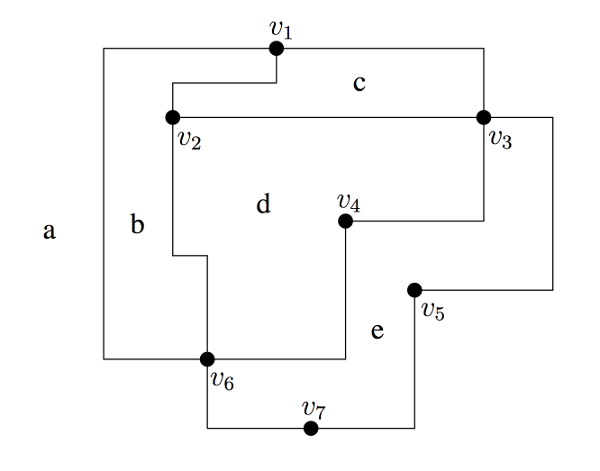
\includegraphics[scale=0.5]{img/fig3.png}
  \end{center}
  \caption{Figure 3 taken from the assignment}
\end{figure*}

In concrete terms, consider Figure 3 from the assignment text (see Figure~\ref{fig:rect-layout}),

